\section{Series Elastic Actuator Control}\label{sec:sea_control}

To control the prosthesis we use Simulink Real-Time (Mathworks, USA), which
samples all sensors (joint encoders, IMU on thigh, force sensors in foot),
computes the desired torques for the knee and ankle joints using a high-level
control strategy, runs the low-level SEA control, which calculates the velocity
of needed to achieve these desired torques, and finally sends the velocity
commands to the motor controllers at a rate of \unit[1]{KHz}. Here, we describe
the low-level SEA control.

First in order to ensure the safety of both the user and the prosthesis, the SEA
controller first saturates the desired torque provided by the high level
controller. During normal operation, we allow a maximum of $\unit[\pm 100]{N
\cdot m}$ of torque at the knee and $\unit[\pm 150]{N \cdot m}$ of torque at the
ankle. Furthermore, when either joint gets within \unit[5]{degrees} of its joint
limits, a software joint limit stop is activated that calculates torques that
prevent the actuator from damaging itself. The joint limit torque is inspired by
the limit torque used in the neuromuscular model simulation presented in
\cref{sec:neuro_mech_model} and takes the form
\begin{align}
    \tau_\tn{lim} = k_\tn{lim} \Delta \theta_\tn{lim} 
    (1 + \nicefrac{\dot \theta_\tn{lim}}{\dot \theta_\tn{max}}) 
    (\Delta \theta_\tn{lim}  > 0) 
    \left(\nicefrac{\dot \theta_\tn{lim}}{\dot \theta_\tn{max}} > -1 \right), 
    \label{eq:tau_joint_limit_pros}
\end{align}
where $k_\tn{lim}$ is the joint limit stiffness, $\Delta \theta_\tn{lim}$ is the
penetration of the joint into the limit region, $\dot \theta_\tn{lim}$ is the
penetration velocity, and $\dot \theta_\tn{max}$ defines the retraction
velocity at which the limit torque drops to zero. The knee extension limit
activates below \unit[5]{degrees} of flexion at which point above torque is
added to the desired torque. The knee flexion limit is set to
\unit[90]{degrees} beyond which the above limit torque saturates the desired
torque from above. For the ankle joint, the extension and flexion activate at
$\unit[\pm 20]{degrees}$ after which the limit torque saturates the desired
torque from below and above respectively. 

Next, to improve the behavior of the prosthesis knee during swing, damping
compensation is added to the desired torque to compensate for friction and
damping in the knee bearing. Finally, after saturation and friction
compensation, a low pass filter is applied to ensure the derivatives of the
desired torque are smooth and to remove frequencies that may excite the SEA
spring. For both joints we use second order Butterworth filters with a cutoff
frequency of \unit[25]{Hz} at the knee and \unit[20]{Hz} at the ankle.

\begin{marginfigure}[-0.0in]
    \centering 
    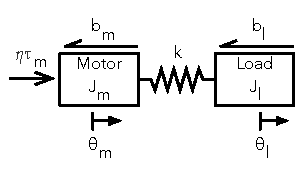
\includegraphics[height=2in]{sea_diagram_ctrl}
    \caption[Dynamics model used to derive sea control]{Dynamics model used to
    derive sea control. $\theta_m$ is the post-gearbox motor angle, $J_m$ and
    $b_m$ are the reflected motor inertia and damping, $\theta_l$ is the load
    angle, $J_m$ and $b_m$ are the load inertia and damping respectively. $k$ is
    the SEA spring stiffness.  $\tau_\tn{m}$ is the motor torque applied to the
    motor rotor and $\eta$ captures the efficiency of the motor torque
    transmission.}\label{fig:sea_diagram_ctrl}
\end{marginfigure}
Next, to achieve the desired torque $\tau_\tn{des}$ in the SEA spring, we
implement an SEA control similar to that used in
\citet{schepelmann2012development}. The control uses proportional feedback to
calculate the desired velocity needed to achieve the desired load torque:
\begin{align}
    \dot \theta_\tn{des} = k_\tn{p} (\tau_\tn{des} - \tau_\tn{meas})
\end{align}
where $\dot \theta_\tn{des}$ is the desired motor velocity and $\tau_\tn{meas}$
is the measured torque. As shown in \cref{fig:sea_diagram_ctrl}, the torque on
the load can be measured through the deflection of the SEA spring as
$\tau_\tn{meas} = k (\theta_\tn{l} - \theta_\tn{m})$ where $\theta_\tn{l}$ is
the position of the load side of the spring and $\theta_\tn{m}$ is the position
of the motor side. To this feed-back control we also add a feed-forward velocity
term. We derive this term by differentiating the desired torque on the load and
solving for the motor velocity
\begin{align}
    \dot \tau_\tn{des} &= k (\dot \theta_\tn{l} - \dot \theta_\tn{m}) \\
    \implies \dot \theta_\tn{m} &= \frac{\dot \tau_\tn{des}}{k} 
        + \dot \theta_\tn{l}.\label{eq:motor_vel_from_tau_des}
\end{align}
Making the total desired velocity,
\begin{align}
    \dot \theta_\tn{des} = k_\tn{p} (\tau_\tn{des} - \tau_\tn{meas}) 
        + \frac{\dot \tau_\tn{des}}{k} + \dot \theta_\tn{l}.
\end{align}

The motor controllers used on the prosthesis (Elmo Motion Control Gold Series)
also accept a feed forward torque command, which can help achieve desired
velocities more quickly. To derive the feed forward motor torque we refer to the
motor dynamics depicted in \cref{fig:sea_diagram_ctrl}. The dynamics of the
motor rotor are
\begin{align}
    \eta \tau_\tn{m} - \tau_\tn{l} - b_\tn{m} \dot \theta_\tn{m} 
        = J_\tn{m} \ddot \theta_\tn{m}
\end{align}
Where $\eta$ is the efficiency of gear set and $\tau_\tn{m}$ is the motor
torque. Solving for the motor torque yields
\begin{align}
    \tau_\tn{m} = \frac{1}{\eta} \left( J_\tn{m} \ddot \theta_\tn{m} 
        + b_\tn{m} \dot \theta_\tn{m} + \tau_\tn{l} \right)
    \label{eq:motor_torque_nosub}
\end{align}
To eliminate the motor velocity and acceleration from the right side of the
equation, we calculate the second derivative of the desired load torque
\begin{align}
    \ddot \tau_\tn{des} &= k (\ddot \theta_\tn{l} - \ddot \theta_\tn{m}) \\
    \implies \ddot \theta_\tn{m} &= \frac{\ddot \tau_\tn{des}}{k} 
        + \ddot \theta_\tn{l},\label{eq:motor_accel_from_tau_des}
\end{align}
and substitute \cref{eq:motor_vel_from_tau_des,eq:motor_accel_from_tau_des} into
\cref{eq:motor_torque_nosub} to arrive at the final feed forward motor torque
\begin{align}
    \tau_\tn{m} = \frac{1}{\eta} \left( J_\tn{m} 
        \left( \frac{\ddot \tau_\tn{des}}{k} + \ddot \theta_\tn{l} \right)
        + b_\tn{m} \left(\frac{\dot \tau_\tn{des}}{k} + \dot \theta_\tn{l}\right)
        + \tau_\tn{l} \right).
\end{align}

The final two steps of the SEA control are to saturate and low pass filter the
desired joint velocities and feed forward motor torques to ensure safety and
suppress excitatory frequencies. Knee velocities are saturated to lie within
$\unitfrac[\pm 9.95]{rad}{sec}$ and ankle velocities are saturated to lie within
$\unitfrac[\pm 6.96]{rad}{sec}$. Furthermore, if a joint violates specified hard
constraint limits, the desired velocities are saturated to zero to prevent
further constraint violation. For the knee joint, the flexion limit is set to
\unit[90]{degrees} and the extension limit is \unit[-2]{degrees}. For the ankle
joint the flexion/extension limits are set to $\unit[\pm 30]{degrees}$
respectively. The saturated desired motor velocities and feed forward motor
torques are then low pass filtered with second order Butterworth filters. For
the knee, we use a cutoff frequency of \unit[100]{Hz} and for the ankle we use a
cutoff frequency of \unit[50]{Hz}.
